\section{Predictive Reconfiguration Control}\label{sec:propose}

\begin{figure}
    \centering
    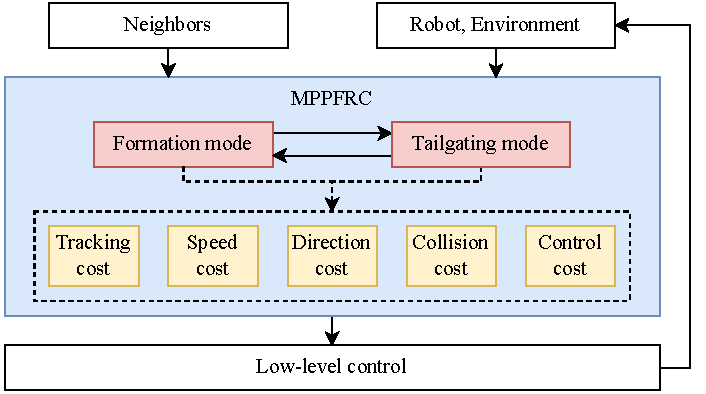
\includegraphics[width=0.7\textwidth]{paper3/images/diagram.pdf}
    \caption{Diagram of the proposed predictive reconfiguration control strategy.}
    \label{fig:diagram}
\end{figure}

The aim of reconfiguration control is to drive the robot swarm through a cluttered environment having narrow passages. The swarm adheres to the following constraints: (\textit{C1}) maintain certain desired shapes; (\textit{C2}) move along a prioritized direction $\mathbf{u}_\text{ref}\in\mathbb{R}^{3}$; (\textit{C3}) obtain the desired speed $\bar{v}_\text{ref}\in\mathbb{R}$; and (\textit{C4}) ensure no collision with other neighbors or obstacles in the environment. To address this problem, we propose a predictive reconfiguration control system as shown in Figure~\ref{fig:diagram}. Inputs to this system include point cloud data from range sensors and the states of neighbor robots. Depending on the environment structure inferred from the point cloud data, the controller operates in either the \textit{``formation''} or \textit{``tailgating''} mode. The \textit{``formation''} mode maintains the desired shape, whereas the \textit{``tailgating''} mode transforms the formation into a line to navigate through narrow spaces like valleys or tunnels. The controller is designed based on a weighted-sum of five cost functions to meet constraints $(C1)-(C4)$. An optimal solver is then used to generate control signals for low-level controllers.

Let $\delta_{ij}\in\mathbb{R}^3,\forall j\in \mathcal{N}_i$ be the vector representing the desired position of robot $i$ with respect to neighbor $j$. The formation is obtained via the following constraint~\cite{Dong2016,6798711}:
\begin{equation}
    \lim_{k\to\infty}{\left(\mathbf{p}_j(k)-\mathbf{p}_i(k)+\kappa\delta_{ij}\right)}=0,\quad\forall i,j\in\{1,...,n\}, i\neq j
\end{equation}
where $\kappa\in[0,1]$ is a scaling factor representing the shrinkage level of the formation. The desired relative position of robot $i$ in the formation is then described as:
\begin{equation}
    \mathbf{p}^*_i(k)=\dfrac{1}{n_i}\sum_{j\in\mathcal{N}_i}{\left(\mathbf{p}_j\left(k\right)+\kappa\delta_{ij}\right)}.
    \label{eqn:formation}
\end{equation}

During the transition between modes, each robot determines a leader as a reference to determine its position. The leader is selected based on the inner product $\tilde{\mathbf{p}}_{ij}$ of the difference between robot $j$ in the neighbor set $\mathcal{N}_i$ and robot $i$, $\mathbf{p}_j-\mathbf{p}_i$, and the desired direction, $\mathbf{u}_\text{ref}$, as follows:
\begin{equation}
    \tilde{\mathbf{p}}_{ij} = \left\langle (\mathbf{p}_j-\mathbf{p}_i),\mathbf{u}_\text{ref}\right\rangle.
    \label{eqn:tildep}
\end{equation}

A positive value of $\tilde{\mathbf{p}}_{ij}$ indicates that robot $j$ is in front of robot $i$ in the $\mathbf{u}_\text{ref}$ direction, and vice versa. Let $\mathcal{P}_i$ be the set of inner products for all robots $j$ in the neighbor set $\mathcal{N}_i$, $\mathcal{P}_i=\left\{\tilde{\mathbf{p}}_{ij}\right\}$. Leader robot ${l_i}$ of robot $i$ is chosen as the closest robot in front of it, i.e.,
\begin{equation}
     l_i=\begin{cases}
    \arg\min_{j}\left\{\tilde{\mathbf{p}}_{ij}\in\mathcal{P}_i\vert\tilde{\mathbf{p}}_{ij}\geq0\right\} & \exists~\tilde{\mathbf{p}}_{ij}\geq0\\ 
    -1 & \text{otherwise}
     \end{cases}
    \label{eqn:li}
\end{equation}

\begin{algorithm}
\caption{Pseudocode of the leader selection}
\label{alg:ls}
\ForEach{$j\in\mathcal{N}_i$}{
    Compute inner product $\tilde{\mathbf{p}}_{ij}$\tcc*[r]{Eq. \ref{eqn:tildep}}
    $\mathcal{P}_i\leftarrow\tilde{p}_{ij}$\;
}
Select leader $l_i$ for robot $i$ to follow\tcc*[r]{Eq. \ref{eqn:li}}
\Return $l_i$\;
\end{algorithm}

Algorithm~\ref{alg:ls} presents the leader selection process. 

In the \textit{``tailgating''} mode, robot~$i$ needs to align and keep a distance~$\bar{d}_\text{ref}\in\mathbb{R}$ with its leader~$l_i$. This can be formulated as follows:
\begin{equation}
    \lim_{k\to\infty}{\left\Vert \mathbf{p}_{l_i}(k)-\mathbf{p}_i(k)\right\Vert}=\bar{d}_\text{ref}
    \label{eqn:tailcon}
\end{equation}
The desired relative position of robot~$i$ then can be determined as follows:
\begin{equation}
    \mathbf{p}_i^*(k)= \mathbf{p}_{l_i}(k)-\bar{d}_\text{ref}\mathbf{u}_\text{ref}.
    \label{eqn:tailgating}
\end{equation}

Using equations \eqref{eqn:tildep} and \eqref{eqn:tailgating}, the formation problem is converted into tracking the desired position $\mathbf{p}_i^*$, which can be handled by predictive controllers. 

\subsection{Predictive control design} 
\begin{figure*}
    \centering
    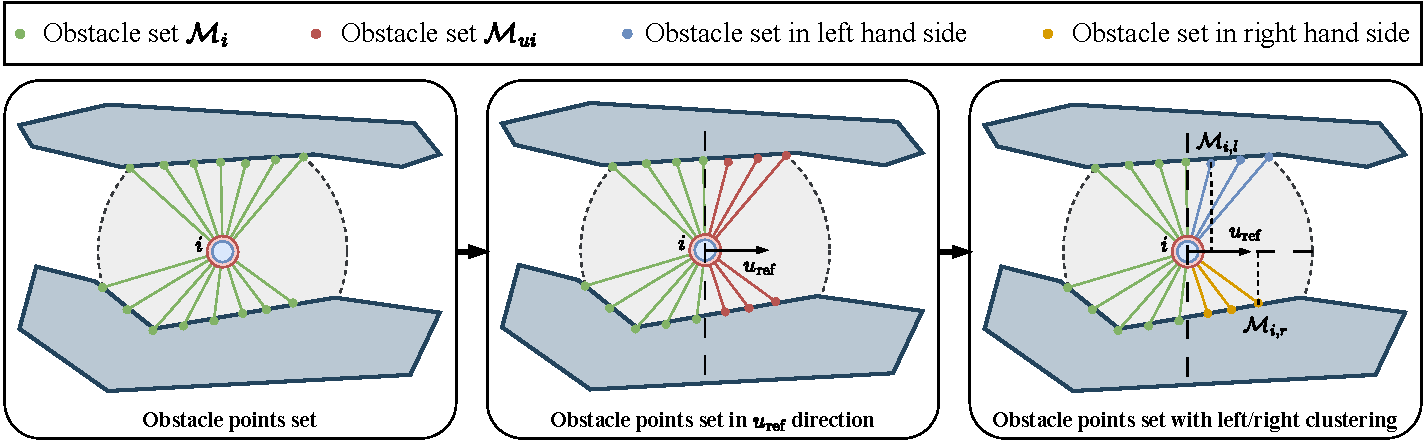
\includegraphics[width=\textwidth]{paper3/images/perception.pdf}
    \caption{The process of estimating the environment's width from the robot's range sensor.}
    \label{fig:perception}
\end{figure*}
The proposed predictive controller uses the desired position $\mathbf{p}_i^*$ as the reference and a set of cost functions to fulfill formation constraints $(C1)-(C4)$. The functions include tracking cost $J_{t,i}$, direction cost $J_{d,i}$, speed cost $J_{s,i}$, obstacle avoidance cost $J_{o,i}$, inter-agent collision cost $J_{i,i}$, and control effort cost $J_{u,i}$. Let $P\in\mathbb{N}^+$ be the prediction horizon, which is finite and shifts forward at each time step; $(\cdot)(k+l|k )$, $l \in\{0,...,P\}$, be the predicted value of $(\cdot)(k+l )$ when the information at time $t(k)$ is available; $\mathbf{X}_i(k)\in\mathbb{R}^{6P}$ be the sequence of the predicted states $\mathbf{x}_i(k+l|k)$ over the horizon $l\in\{1,...,P\}$; and $\mathbf{U}_i(k)\in\mathbb{R}^{3P}$ be the sequence of the predicted control inputs $\mathbf{u}_i(k)$ over the horizon $l\in\{0,...,P-1\}$. The predictive reconfiguration control can be modeled as a non-convex optimization problem as follows:
\begin{equation}
    \min_{\mathbf{U}_i(k)}\left(J_{t,i}(k)+J_{s,i}(k)+J_{d,i}(k)+J_{o,i}(k)+J_{i,i}(k)+J_{u,i}(k)\right)
    \label{eqn:J}
\end{equation}
subject to:
\begin{equation}
    \begin{aligned}
        &\mathbf{x}_i(k+l+1|k)=\mathbf{A}\mathbf{x}_i(k+l|k)+\mathbf{B}\mathbf{u}_i(k+l|k),\\
        &\mathbf{x}_i(k|k)=\mathbf{x}_i(k),\\
        &\mathbf{v}_\text{min}\leq \mathbf{v}_i(k+l|k)\leq \mathbf{v}_\text{max},\\
        &\mathbf{u}_\text{min}\leq \mathbf{u}_i(k+l|k)\leq \mathbf{u}_\text{max},\\
    \end{aligned}
    \label{eqn:constraints}
\end{equation}
with $l\in\{1,...,P\}$, and $i\in\mathcal{N}$. The cost functions are defined as follows.

\subsubsection{Tracking cost}\label{sec:tracking_term}
The tracking term aims to drive the robots toward their reference positions to achieve the desired formation shape. It is defined as the square error between the desired position~$\mathbf{p}_i^*$ and the predicted position~$\mathbf{p}_i$ of robot $i$ as follows:
\begin{equation}
    J_{t,i}(k)=w_t\sum_{l=1}^P{\left\Vert \mathbf{p}^*_i(k+l|k)-\mathbf{p}_i(k+l|k)\right\Vert^2},
\end{equation}
where $w_t$ is a positive tracking weight.

\subsubsection{Speed cost}
The speed cost is used to maintain the desired speed $\bar{v}_\text{ref}$ of the swarm. It is defined as the squared difference between the actual and the desired speed of the robots as follows:
\begin{equation}
    J_{s,i}(k)=w_s\sum_{l=1}^P\left(\left\Vert \mathbf{v}_i(k+l|k)\right\Vert^2-\bar{v}_\text{ref}^2\right)^2,
\end{equation}
where $w_s$ is a positive weight.

\subsubsection{Direction cost}
This cost directs the robots to move in the desired direction $\mathbf{u}_\text{ref}$. It is computed based on the normalized dot product between velocity $\mathbf{v}_i$ and the desired direction $\mathbf{u}_\text{ref}$ of robot $i$. It is equal to zero when the velocity perfectly aligns with the reference direction and otherwise increases proportionally with the degree of misalignment. It is given as follows:
\begin{equation}
    J_{d,i}(k)=w_d\sum_{l=1}^P{\left(1-\dfrac{\left\langle \mathbf{v}_i\left(k+l|k\right),\mathbf{u}_\text{ref}\right\rangle^2}{\left\Vert \mathbf{v}_i(k+l|k)\right\Vert^2}\right)^2},
\end{equation}
where $w_d$ is a positive direction weight.

\subsubsection{Collision avoidance cost}
To avoid collisions, the distance from a robot to any obstacle must be greater than the robot's radius $r$ and the distance between any two robots must be greater than $2r$. Let $d_{ij}=\left\Vert \mathbf{p}_j-\mathbf{p}_i\right\Vert$ be the distance between robots $i$ and $j$, and $d_{im}$ be the distance between robot $i$ and obstacle $\mathbf{m}$. The constraints for collision avoidance  are given as follows:
\begin{equation}
\begin{aligned}
    d_{im}(k+l|k)&\geq r \quad i\in\mathcal{N}, \mathbf{m}\in\mathcal{M}_i(k)
    \label{eq:obsContraint}
\end{aligned}
\end{equation}
\begin{equation}
\begin{aligned}
    d_{ij}(k+l|k)&\geq 2r \quad i\in\mathcal{N},j\in\mathcal{N}_i
    \label{eq:robotContraint}
\end{aligned}
\end{equation}

In this work, constraint (\ref{eq:obsContraint}) is represented via obstacle avoidance cost $J_{o,i}$ defined as a logistic function as follows~\cite{8202163}:   

\begin{equation}
    J_{o,i}(k) = w_o\sum_{l=1}^P \dfrac{1}{1 + \exp{\left(\alpha\left(d_{im}^\text{min}(k+l|k) - r\right)\right)}},
\end{equation}
where $w_o > 0$ is a constant weight, $\alpha > 0$ is a smoothness parameter, and
\begin{equation}
    d_{im}^\text{min}(k+l|k)=\min\left\{d_{im}(k+l|k)|\mathbf{m}\in\mathcal{M}_i\right\}.
\end{equation}

Similarly, constraint (\ref{eq:robotContraint}) is represented via an inter-agent collision cost $J_{i,i}$ defined as follows~\cite{736776}:
\begin{equation}
    J_{i,i}(k)=\dfrac{w_i}{n_i}\sum_{l=1}^P{\sum_{j\in\mathcal{N}_i}}F_{ij}(k+l|k),
\end{equation}
where $w_i>0$ is a constant weight and  
\begin{equation}
    F_{ij}(k+l|k)=\begin{cases}
        0   & \text{if } d_{ij}(k+l|k) \geq \beta r\\
        \dfrac{\beta r-d_{ij}(k+l|k)}{(\beta-2)r}    & \text{if } 2r < d_{ij}(k+l|k) < \beta r\\
        \infty  & \text{if } d_{ij}(k+l|k) \leq 2r
    \end{cases}
\end{equation} 
with $\beta>2$ being the influence ratio of the neighbors.

\subsubsection{Control effort cost}
The control effort cost is used as a penalty term to minimize the control signal. It is defined as:
\begin{equation}
    J_{u,i}(k)=w_u\sum_{l=0}^{P-1}\left\Vert \mathbf{u}_i(k+l|k)\right\Vert^2,
\end{equation}
where $w_u>0$ is a constant control weight.

\subsection{Formation reconfiguration}\label{sec:obs_aware}

Depending on the environment's width, the control system can determine the formation shape and scaling factor $\kappa$. The process of estimating the environment's width is illustrated in Figure~\ref{fig:perception}. Robot $i$ first obtains point cloud data $\mathcal{M}_i$ (green) from its local sensor and then selects a point set $\mathcal{M}_{ui}$ (red) in front of the robot along the moving direction $u_\text{ref}$ as follows:
\begin{equation}
    \mathcal{M}_{ui} = \left\{\mathcal{M}_{i}\vert\left\langle\left(\mathbf{p}_i-\mathcal{M}_{i}\right),u_\text{ref}\right\rangle<0\right\}.
    \label{eqn:mui}
\end{equation}
The DBSCAN algorithm~\cite{10.5555/3001460.3001507} is then used to divide $\mathcal{M}_{ui}$ into two clusters corresponding to the left (blue) and right (yellow) sides of the robot. Data points $\mathcal{M}_{i,l}$ and $\mathcal{M}_{i,r}$ from those clusters with the shortest distance to $u_\text{ref}$ are then selected. Using these points, the environment's width is computed as:
\begin{equation}
    w_e= \left\Vert\left(\mathcal{M}_{i,r}-\mathcal{M}_{i,l}\right)\times \mathbf{u}_\text{ref}\right\Vert
    \label{eqn:we}
\end{equation}
The pseudocode to estimate the environment's width is presented in Algorithm~\ref{alg:we}. 

On the other hand, the formation's width $w_f$ is predefined for each specific formation shape. The scaling factor $\kappa$ then can be computed based on the environment's and formation's width as follows:
\begin{equation}
    \kappa = 
    \begin{cases} 
        \dfrac{w_e - 2r}{w_f} & \text{if } w_e \geq \lambda r \\
        0 & \text{otherwise}
    \end{cases}
    \label{eqn:kappa}
\end{equation}
where $\lambda > 2$ is a scaling coefficient determining the environment's width at which the PRC switches its mode. 

\begin{algorithm}[h!]
\caption{Pseudocode to estimate the environment's width}
\label{alg:we}
Get point set $\mathcal{M}_{ui}$ in front of robot $i$ in moving direction $\mathbf{u}_\text{ref}$\tcc*[r]{Eq. \ref{eqn:mui}}
Cluster $\mathcal{M}_{ui}$ for the left and right sides of the robot using DBSCAN\;
Find point pair $\left(\mathcal{M}_{i,l},\mathcal{M}_{i,r}\right)$, whose distance to $\mathbf{u}_\text{ref}$ is minimum\;
Compute the environment's width $w_e$\tcc*[r]{Eq. \ref{eqn:we}}
\Return $w_e$\;
\end{algorithm}

\begin{algorithm}[h!]
\caption{Pseudocode of the PRC}
\label{alg:our}
Get data point set $\mathcal{M}_i$\;
\If{$\mathcal{M}_i$ is empty}{
    mode $\leftarrow$ \textit{``formation''}\;
    $\kappa \leftarrow 1.0$\;
}
\Else{
    Get the environment's width $w_e$\tcc*[r]{Alg. \ref{alg:we}}
    \If{$w_e$ is None}{
        mode $\leftarrow$ \textit{``formation''}\;
        $\kappa \leftarrow 1.0$\;
    }
    \Else{
        \If{$w_e\leq\lambda r$}{
            mode $\leftarrow$ \textit{``tailgating''}\;
        }
        \Else{
            mode $\leftarrow$ \textit{``formation''}\;
            Estimate the desired formation width $w_f$\;
            \If{$w_e-2r\leq w_f$}{
                Compute the scaling factor $\kappa$\tcc*[r]{Eq. \ref{eqn:kappa}}
            }
            \Else{
                $\kappa\leftarrow1.0$\;
            }
        }
    }
}
\Switch{mode}{
\Case{``formation''}
{
    Get the desired position $\mathbf{p}_i^*$\tcc*[r]{Eq. \ref{eqn:formation}}
}
\Case{``tailgating''}
{
    Select a leader to follow\tcc*[r]{Alg. \ref{alg:ls}}
    Get the desired position $\mathbf{p}_i^*$\tcc*[r]{Eq. \ref{eqn:tailgating}}
}
}
Establish the formation cost function\tcc*[r]{Eqs. \ref{eqn:J}-\ref{eqn:constraints}}

Minimize the cost function to obtain the optimal control signal $\mathbf{u}_i^*$\tcc*[r]{MPC solver~\cite{2020SciPy-NMeth}}

\Return $\mathbf{u}_i^*$\;
\end{algorithm}

Algorithm~\ref{alg:our} presents the pseudocode of the PRC. At each time step, the system estimates the width of the environment to determine the formation mode and the scaling factor $\kappa$. It then computes the desired position $\mathbf{p}_i^*$ for each robot and establishes the formation cost function using equations \eqref{eqn:J} - \eqref{eqn:constraints}. This problem is then solved to find the optimal control signal $\mathbf{u}_i^*$ using common nonlinear programming (NLP)
solvers, such as the Sequential Least Squares Programming (SLSQP)~\cite{kraft1988software}. In this work, we implemented the solver in Python using the optimization software library SciPy~\cite{2020SciPy-NMeth}.